\documentclass[11pt]{article}
\usepackage{xargs}                      % Use more than one optional parameter in a new commands
\usepackage{xcolor}  % Coloured text etc.
\usepackage{pgfgantt}
\usepackage{mathtools}
\usepackage{hyperref}
\usepackage{float}
\usepackage[toc,page]{appendix}
\usepackage[british]{babel}
\usepackage[bibstyle=numeric, backend=biber, sorting=none]{biblatex}
\addbibresource{../Meine Bibliothek.bib}
% 
\usepackage[colorinlistoftodos,prependcaption,textsize=tiny]{todonotes}

\newcommand{\defeq}{\vcentcolon=}
\newcommandx{\unsure}[2][1=]{\todo[linecolor=red,backgroundcolor=red!25,bordercolor=red,#1]{#2}}
\newcommandx{\change}[2][1=]{\todo[linecolor=blue,backgroundcolor=blue!25,bordercolor=blue,#1]{#2}}
\newcommandx{\info}[2][1=]{\todo[linecolor=OliveGreen,backgroundcolor=OliveGreen!25,bordercolor=OliveGreen,#1]{#2}}
\newcommandx{\improvement}[2][1=]{\todo[linecolor=Plum,backgroundcolor=Plum!25,bordercolor=Plum,#1]{#2}}
\newcommand{\code}[1]{\texttt{#1}}
%Gummi|065|=)
\title{\textbf{Exposé Masterarbeit}}
\author{Carsten Csiky}
\date{}
\begin{document}

\maketitle

\section{Exposition}

\subsection{Why?}

In systems programming, there has always been an interest in both performance and correctness, as 
these pieces of software are often the foundation of critical infrastructure.

The classical approaches to ensure correctness include extensive testing, long experience and bmc, because these approaches are approachable to programmers as well as understandable in the programming context (i.e. no separate language)

Rust -- a relative newcomer to the systems programming field -- has the goal of guaranteeing memory and thread safety at runtime by extending the type system, which works quite well.

User-defined functional requirements however cannot be checked by Rust's type system and require users to use testing / fuzzing to check for correctness.

Testing is inadequate in terms of accuracy, while heavy verification systems are inadequate in terms of accessability to developers:
Both workflow and the specification languages are hard to adapt to existing programming workflows.

In contrast developers are used to interacting with statically typed languages and their type warnings. It is therefore desirable to embed functional verification systems in type checking phase a compiler.


% Programming paradigms have changed over time. Object oriented programming languages like java are popular, but limitations have become apparent.

% As a result functional programming (FP) features have become popular in object-oriented programming languages. The introduction of Java 8's lambda expressions and the new stream interface show, that these features will become more adopted. Increasing the need for KeY to be able to verify them.

% FP features can also be an opportunity for verification, which can benefit from this change: Smart specification and use of FP features can ease the specification and verification burden for an API consumer. Since FP for example could replace many for-loops, the burden of specifying loop invariants and prooving termination can be shifted to the definition and done once, instead of repeating the same steps for every for-loop. FP in java could thus lead to easier and faster verification.

% To ensure the usefullness of the KeY verification tool for the future, it is therefore key to support FP features.

\subsection{What?}


The thesis will enable automated verification of Rust programs against refinement type specifications.

The verification should be sound, decidable and feasible in the identified use cases, which will be tested on minimal -- yet representative -- examples. The examples will include full refinement type annotations, consequently making type inference optional.

The specification will be written in an extension of the Rust type language, inspired by refinement types.

\subsection{How?} \label{ssec:How}

This section starts with outlining the fundamental ideas (denoted "I1" to "I4") the thesis will be based on.

\begin{itemize}
	\item[I1] adapt Refinement Type semantics to Rust, especially for mutability in Rust's Ownership Model
	\item[I2] Treat owner and immutable types as logical variables (i.e. referentially transparent, unchanging)
	\item[I3] Treat mutable references as state transitions from start of end of borrow
	\item[I2] develop a prototype for translating refinement type judgments to a verification backend (e.g. z3, prusti)
	\item[I3] conduct a feasibility study on different categories of common use cases
	% \item[I1] reuse features already implemented in KeY (namely model methods and method verification)
	% \item[I2] treat Lambdas as explicit Classes
	% \item[I3] define contracts using KeY's Model Methods
	% \item[I4] transform lambda specifications into method contracts
	% \item[I5] feasibility study on different categories of common use cases
\end{itemize}

The following enumeration lists the concrete tasks (denoted "T1" to "T6") with their respective deliverable. These tasks are connected to specific time in Section \ref{sec:schedule}.

\begin{itemize}
	\item[T1] \label{itm:T1} identify common use cases for refinement types and categorize them, in particular use cases with mutable references. The deliverable is a set of minimal -- yet representative -- examples, with explanations for why they are representative.
	\item[T2] devise a system for type specifications, which would ideally cover the identified use cases. Refinement types are inherently limited in expressiveness, thusly in cases where use cases cannot be covered, the reason will be explained. The result is a concrete description of the syntax and type judgment semantics.
	\item[T3] implement a parser for the refinement language defined above. The product is a parser that can parse the refinement language.
	\item[T4] transform refinement types and Rust AST to a verification backend. The product is an implementation, or alternatively a description of the process.
	\item[T5] if necessary for the use cases, a definition of suitable axioms for language build-in types. The deliverable is a set of refinement type coercions.
	\item[T6] conduct a feasibility study on the examples of the use cases in \hyperref[itm:T1]{T1}. The result is a set of proven examples. If some examples could not be proven, the reason will be investigated and explained.
\end{itemize}


\section{Defining the Goal}

The goal of the thesis is to show that Refinement Types can be idiomatically adapted to mutable languages when leveraging a strong Ownership Model. It aims to enable gradual adoption of lightweight verification methods to Rust.

I aim for automated parsing of refinement types and verification. As well as giving a description of the syntax and semantics of the constructs, that will extend Rust's type system.

A feasibility study on the previously defined use cases will show how useful the proposed additions are. For use cases that could not be covered by the proposed additions, the reason will be investigated.
In case implementing these translations could not be completed, the use cases will be transformed manually.

Specifying or verifying complete Rust modules or the entire Rust language is not the goal of the thesis.

In particular \code{unsafe} Rust will not be represented in the specification nor implementation.

\todo{Define subset or Rust?}

Implementing liquid type inference in also not a goal of the thesis.

\section{State of the Art}

There currently does not exist an implementation of refinement types for Rust.

Relevant papers originate from two lines of work. Firstly additions to refinement types for mutability, asynchronous execution etc. and secondly other verification frameworks for Rust.

For example, Lanzinger \cite{lanzinger_property_2021} successfully adapted refinement types to Java, which allows the user to check, that property types described by java annotations hold true throughout the program. At this point in time, specification and verification is limited to immutable (\code{final}) data.

Kloos et al. \cite{kloos_asynchronous_2015} extended refinement types to mutable and asynchronous programs. The paper explores how changes to possibly aliased memory cells can be tracked throughout a OCaml program. For that purpose the types are extended by a set of requirements on memory objects, which track distinctness and refined types of these memory cells. In contrast to OCaml, Rust already guarantees that mutable memory is not aliased and in particular \textit{all mutable memory locations must be accessible by a variable name in the current context}, which offers substantial advantages in terms of simplicity to specification and verification of Rust programs.

In terms of alternative verification approaches, Prusti\cite{astrauskas_leveraging_2019} is notable, because of their work on formalizing the full Rust semantics, including \code{unsafe}. Prusti is a heavy-weight functional verification framework for Rust; based on separation logic.

Alternative verification approaches also exists: For example RustHorn\cite{matsushita_rusthorn_2020} employs constrained horn clauses based verification to Rust. Particularity relevant for this thesis is the novel formalization for mutable references used in the paper. The authors stipulate that mutable references should be specified by a pre- and post-state from before a reference is borrowed to after it is returned.

\section{Schedule} \label{sec:schedule}

This sections describes the relation of the tasks from Section \ref{ssec:How} to their timeslot and the dependencies between them in form of a gantt diagram. There are two milestones: Completion of Specification (denoted \textit{Specification}) and the completion of implementation (denoted \textit{Implementation}).

\begin{ganttchart}[
	time slot format=isodate,
	x unit=0.04cm,
	today = 2022-02-30,
	link bulge=2.5,
	]{2022-02-30}{2022-08-31}
\gantttitlecalendar{year, month=name} \\
\ganttbar{T1 (Use Cases)}{2022-02-30}{2022-03-07} \\
	\ganttlinkedbar[name=T2]{T2 (Formalization)}{2022-03-07}{2022-05-17} \\
		\ganttlinkedmilestone[name=Spec]{Specification}{2022-05-17} \\
			\ganttlinkedbar[name=T5]{T5 (Axioms)}{2022-05-31}{2022-06-15} \\
				\ganttlinkedbar[name=T6]{T6 (Evaluation)}{2022-07-31}{2022-08-15} \\

\ganttbar[name=T3]{T3 (Parsing)}{2022-04-07}{2022-05-07} \\
	\ganttlinkedbar[name=T4]{T4 (Translation)}{2022-05-07}{2022-06-31} \\
		\ganttlinkedmilestone[name=Impl]{Implementation}{2022-07-10} \\

\ganttlink[link mid=0.9]{T3}{Impl}


\ganttbar[name=raw_version]{Draft Version}{2022-06-01}{2022-08-01} \\
	\ganttlinkedbar[name=corrections]{Revisions}{2022-08-01}{2022-08-20} \\
		\ganttlinkedbar{Buffer}{2022-08-20}{2022-08-31} \\
\end{ganttchart}

\newpage
\begin{appendices}

\section{Use Case Analysis}

To gain some understanding of how relevant mutability is in Rust, all published Rust crates (Rusts version packages) published on crates.io with at least 10 versions were analysed\footnote{The limit of 10 versions is used to eliminate inactive and placeholder packages}. The analysis uses the syntactical structure to infer mutability information about the following various AST items: 
\begin{itemize}
	\item Local Variable Definitions. These can be tracked with high confidence
	\item Parameters, which are considered immutable if they are passed as immutable references or owned.
	\item Function Definitions, which are considered immutable, iff all parameters considered immutable.
	\item Arguments. Hard to track
	\item Function Calls, which are considered immutable, iff all arguments are considered immutable.
\end{itemize}
A total of around 52 million items were found in 228263 files in a combined code-base size of over 64 million lines of Rust code (without comments and white space lines)\footnote{Calculated with \texttt{cloc}}

% from cloc
% ----------------------------------------------------------------------------------------
% Language                              files          blank        comment           code
% ----------------------------------------------------------------------------------------
% Rust                                 228263        5664979       10317162       64193670
% C                                     32945        1539542        1979846       13468919
% C++                                   18084        1263696        1093652        7956897
% JSON                                  15838           1897              0        6424252
% C/C++ Header                          31619        1152322        2015896        6284146
% XML                                    5142          25277          25773        4807556
% Assembly                               4146         534785         582345        2631991


Figure~\ref{fig:mutabillity_by_category} shows the ratio of mutable to immutable items. Note that about 30\% of local variables are defined mutable while just 10\% to 20\% of parameters are mutable and less than 10\% of functions have mutable parameters at all.

\begin{figure}[H]
	\centering
	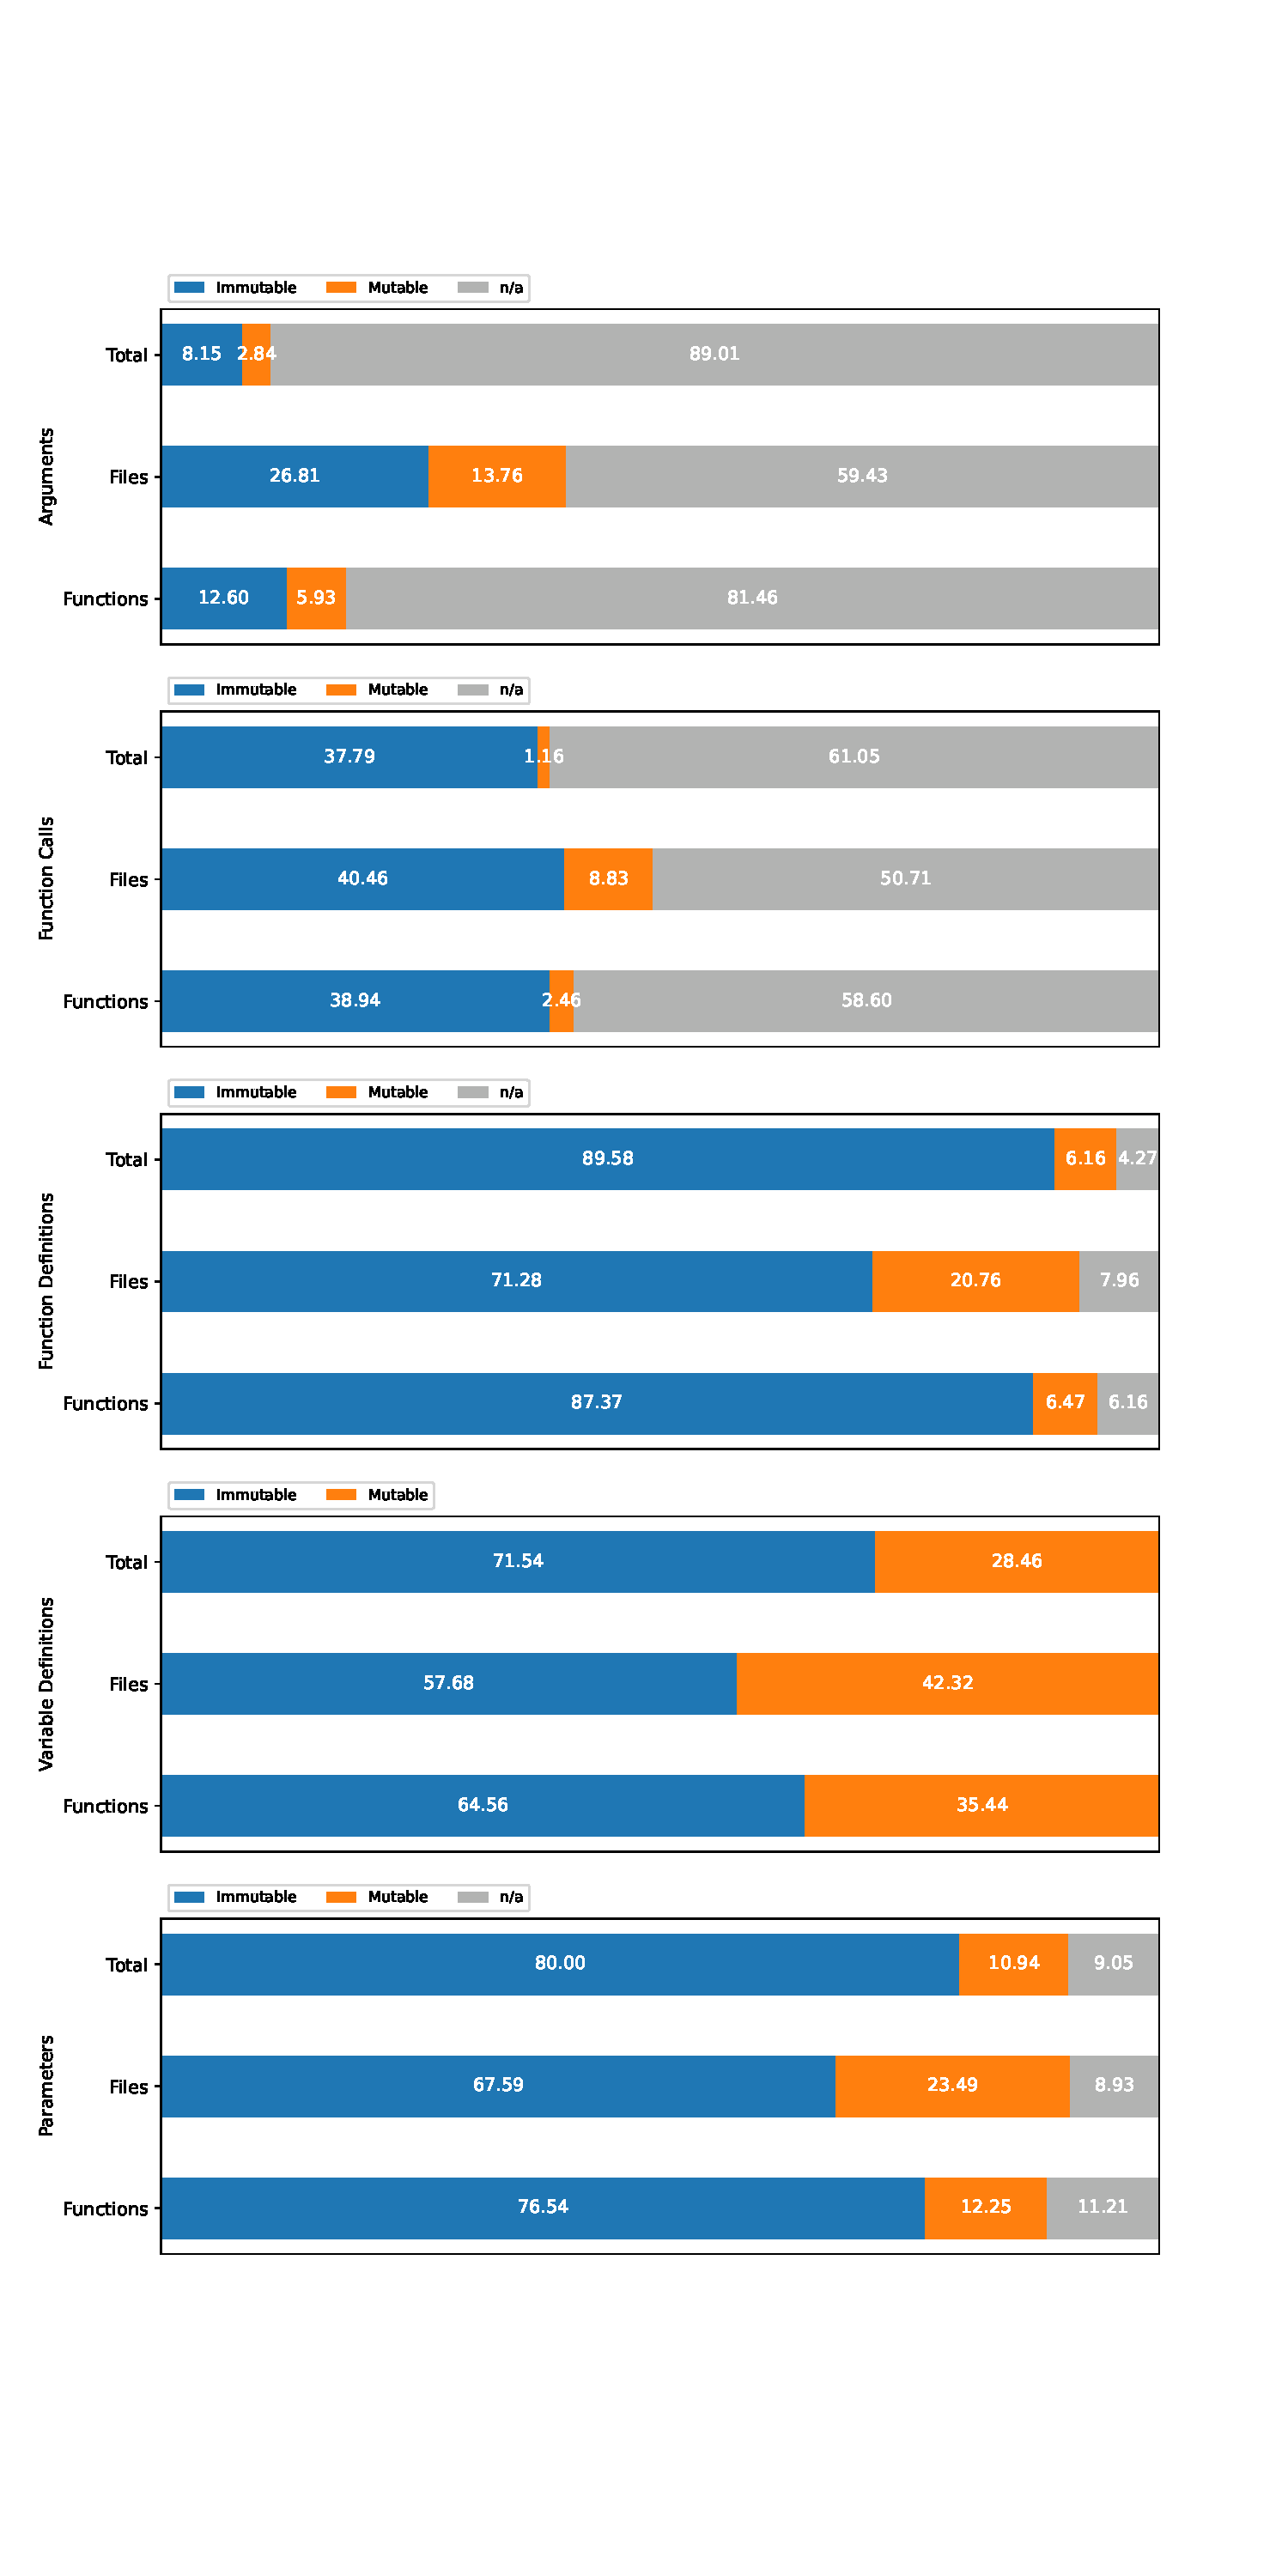
\includegraphics[width=0.9\linewidth, clip, trim={0.5cm 6cm 0.5cm 6cm}]{../mutability_by_category.pdf}
	\caption{Ratio of Immutable to Mutable Versions of Different AST Items. Items are Counted by Unique Occurrences}
	\label{fig:mutabillity_by_category}
\end{figure}


\end{appendices}


\printbibliography

\end{document}
